\begin{figure}[tbp]
\centering
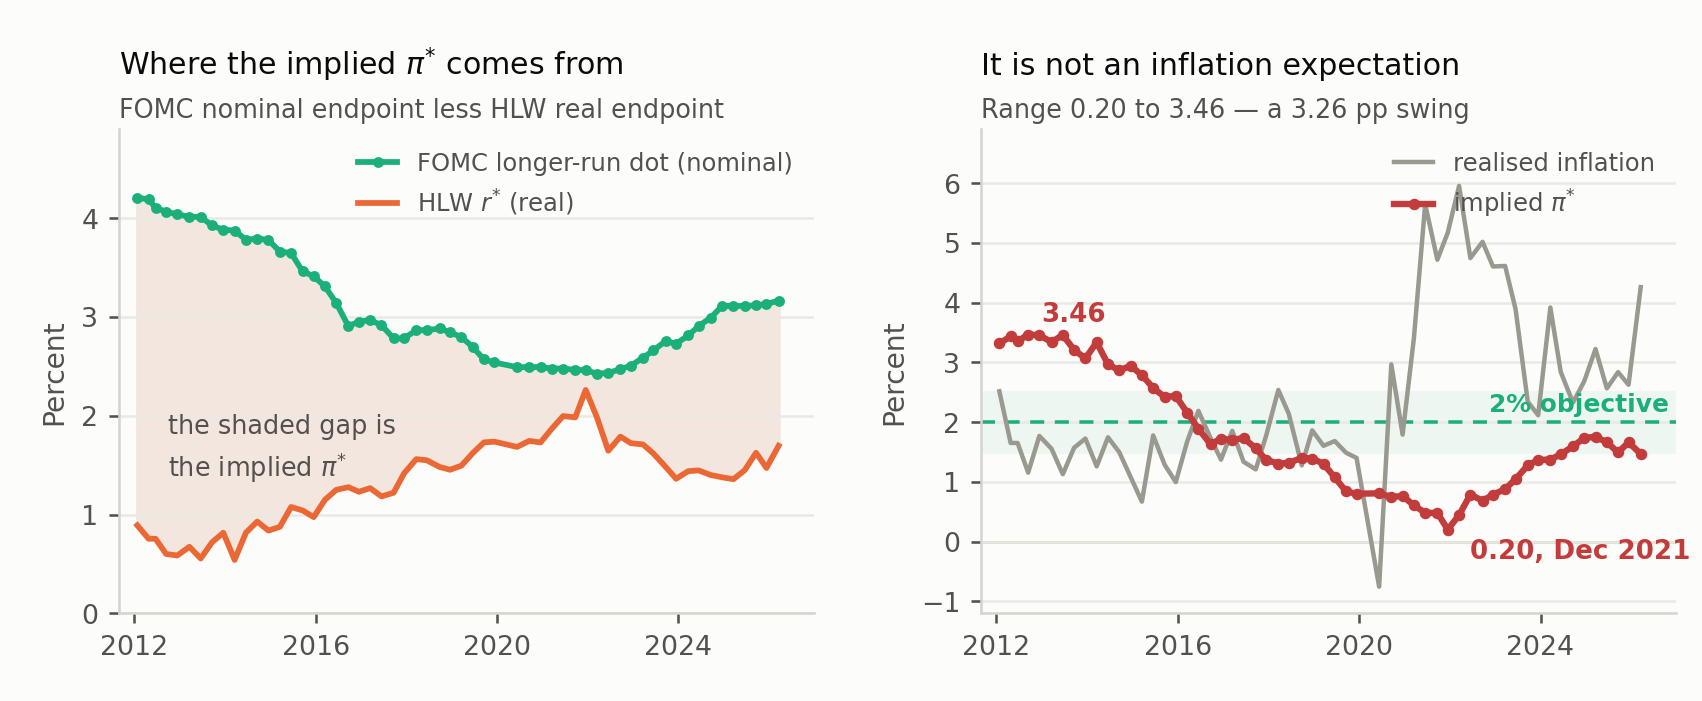
\includegraphics[width=0.95\textwidth]{s_implied_pi.png}
\caption{\textbf{The inflation expectation needed to reconcile the two estimates.} Left: the
FOMC's longer-run federal funds projection, which is nominal, against HLW's one-sided $r^{*}$,
which is real, at the 57 SEP meetings; the shaded area between them is the long-run inflation
expectation that would have to be embedded in the FOMC's projection for the two series to be
mutually consistent. Right: that implied series plotted against realised inflation, with the
2\% objective marked and a 1.5--2.5\% band shaded. The implied series runs from 3.46\% in
September 2012 to 0.20\% in December 2021 --- a swing of 3.26 pp --- and lies outside the
1.5--2.5\% band at 75\% of meetings. At its trough it requires FOMC participants to have
expected 0.20\% inflation in the long run at a moment when realised inflation was 5.17\%. A
mismatch in deflators therefore cannot account for the divergence in
Figure~\ref{fig:rstartwo}: whatever separates the two estimates, it is not the 2\% netting.
Realised inflation is HLW's own four-quarter input series rather than headline PCE.}
\label{fig:impliedpi}
\end{figure}
